% % First, we look at the effects of $c_{xy}$ and $c_{yx}$ on the critical points of \equationautorefname~\eqref{eq:AutonomousSystemODEs}.
% Before, finding the critical points of the system of ODEs, we fix the parameter, $T$, to the optimal temperature, $12.5^{\circ}$C, to eliminate the effect of temperature on the salmon population.
% Now, the equations can be rewritten as:
% \begin{equation}
%     \begin{aligned}
%     \frac{dx}{dt} &= R(T_{opt})x -\frac{R(T_{opt})x^2}{K_x} - c_{xy}xy,\\[.4cm]
%     \frac{dy}{dt} &=r_yy -\frac{r_yy^2}{K_y} + c_{yx}xy.
%     \end{aligned}
% \end{equation}
% Then, substituting $ a_x = R(T_{opt})$, $\displaystyle b_x = \frac{R(T_{opt})}{K_x}$, $a_y = r_y$, and $\displaystyle b_y = \frac{r_y}{K_y}$ a similar model to Theodore Modis' model, \equationautorefname~\eqref{eq:modislotkavoltera}, is constructed.
% Before beginning the analysis of \equationautorefname~\eqref{eq:AutonomousSystemODEs}, values must be assigned to $c_{xy}$ and $c_{yx}$.
% First, we will develop a criteria for these parameters such that the solutions will reflect their behavior.
% We know that the model should be stable near its critical points because if they were unstable, the populations could approach infinity.
% Second, the populations of the species should be oscillating as can be seen in \tablename~\ref{tab:runvsweight}.
% To achieve a stable oscillation at a critical point, we will evaluate the solutions to the model when the eigenvalues for the critical point have non-positive real parts and imaginary parts.

% Since \equationautorefname~\eqref{eq:AutonomousSystemODEs} is non-autonomous, then we can't evaluate it's fixed points.
% So, replacing the salmon model with \equationautorefname~\eqref{eq:salmonlogisticrepo}, and fixing $T=T_{opt}$, produces the below autonomous model.
% \begin{equation}\label{eq:THENonModel}
%     \begin{aligned}
%     \frac{dx}{dt} &= \ln{(R(T_{opt}))}x\left(1-\frac{x}{K_x}\right) - c_{xy}xy,\\[.4cm]
%     \frac{dy}{dt} &=ry\left(1-\frac{y}{K_y}\right) + c_{yx}xy.
%     \end{aligned}
% \end{equation}
% Fixing $T$ to the constant, $T_{opt}$, eliminates the effect of temperature on the salmon population.
% Applying the distributive property to the above system of equations generates the following equations.
% \begin{equation*}
%     \begin{aligned}
%     \frac{dx}{dt} &= \ln{(R(T_{opt}))}x -\frac{\ln{(R(T_{opt}))}x^2}{K_x} - c_{xy}xy,\\[.4cm]
%     \frac{dy}{dt} &=r_yy -\frac{r_yy^2}{K_y} + c_{yx}xy.
%     \end{aligned}
% \end{equation*}
% Then, substituting $ a_x = \ln(R(T_{opt}))$, $\displaystyle b_x = \frac{\ln(R(T_{opt}))}{K_x}$, $a_y = r_y$, and $\displaystyle b_y = \frac{r_y}{K_y}$ a similar model to Theodore Modis' model, \equationautorefname~\eqref{eq:modislotkavoltera}, is constructed.
% \begin{equation}\label{eq:AutonomousSystemODEsModis}
%     \begin{aligned}
%     \frac{dx}{dt} &= a_xx - b_xx^2 - c_{xy}xy,\\
%     \frac{dy}{dt} &= a_yy - b_yy^2 + c_{yx}xy.
%     \end{aligned}
% \end{equation}
% Now, we set the above system of equations equal to the $\Vec{0}$.
% \begin{equation*}
%     \begin{aligned}
%     0 &= x(a_x - b_xx - c_{xy}y),\\
%     0 &= y(a_y - b_yy + c_{yx}x).
%     \end{aligned}
% \end{equation*}
% Then, solving for $x$ and $y$ produces the critical points below.
% \begin{equation*}
%     \begin{array}{ll}
%          x^*_1 = 0, & y^*_1 = 0,  \\
%          x^*_2 = K_x, & y^*_2 = 0,\\
%          x^*_3 = 0, & y^*_3 = K_y,
%     \end{array}
% \end{equation*}
% \begin{equation*}\scalebox{1.2}{$
%     \begin{array}{ll}
%         x^*_4 = \frac{a_xb_y-c_{xy}a_y}{c_{xy}c_{yx}+b_xb_y} & y^*_4 = \frac{a_xc_{yx}+b_xa_y}{c_{xy}c_{yx}+b_xb_y}.
%     \end{array}$}
% \end{equation*}
The first three critical points do not contain either of our unknown parameters, $c_{xy},\;c_{yx}$, but the fourth critical value does.
% Note, neither population can be negative and $c_{xy},\;c_{yx}>0$, which creates the below criteria for these parameters.
% \begin{equation*}\scalebox{1.2}{$
% \begin{array}{c}
%      0<c_{xy} \leq \frac{a_xb_y}{a_y}, \\[.1cm]
%      c_{yx} \geq -\frac{b_xa_y}{a_x}.
% \end{array}$}
% \end{equation*}
% Since $a_x,\;b_x,\;a_y>0$, then the criteria above changes to:
% \begin{equation*}\scalebox{1.2}{$
% \begin{array}{c}
%      0<c_{xy} \leq \frac{a_xb_y}{a_y}, \\[.1cm]
%      c_{yx} > 0.
% \end{array}$}
% \end{equation*}
% If we assume that $c_{yx}>c_{xy}$, this would imply that the rate at which salmon affect brown bears is higher than the rate at which brown bears affect salmon. 
% However, brown bears eat a large quantity of salmon, but salmon do not have this direct impact on bears.
% So, the brown bear population should have a higher affect on the salmon population.
% Therefore, the constraint for the parameters $c_{xy}$ and $c_{yx}$ is as follows.
% \begin{equation*}
%     \begin{array}{c}
%          0<c_{xy}\leq \frac{a_xb_y}{a_y} = 0.104,  \\
%          0<c_{yx}<c_{xy}.
%     \end{array}
% \end{equation*}
% Now, assessing the eigenvalues of \equationautorefname~\eqref{eq:AutonomousSystemODEsModis} with the above constraint, will determine the stability around the critical point $(x^*_4,\;y^*_4)$~\cite{roussel2019stability}.
% The eigenvalues can be found by solving for the characteristic polynomial of the Jacobian matrix for \equationautorefname~\eqref{eq:AutonomousSystemODEsModis}~\cite{roussel2019stability}.
% \begin{equation}\label{eq:Jacobian}
%     J_{(x,y)} =
%     \begin{pmatrix}
%         a_x - 2b_xx -c_{xy}y & -c_{xy}x\\
%         c_{yx}y & a_y - 2b_yy + c_{yx}x
%     \end{pmatrix}.
% \end{equation}
% The characteristic polynomial of the above Jacobian matrix is displayed below.
% \begin{align}
% \begin{split}\label{eq:CharacteristicEq}\displaystyle
%     \text{det}(J_{(x,y)}-\lambda I) = \lambda^2 - \pmb{\big[}\; (a_x - 2b_xx -c_{xy}y) + (a_y - 2b_yy + c_{yx})\;\pmb{\big]}\lambda\\
%     + \pmb{\big[}\; (a_x - 2b_xx -c_{xy}y)(a_y - 2b_yy + c_{yx}) + c_{xy}xc_{yx}y\;\pmb{\big]}.
% \end{split}
% \end{align}
% Note that:
% \begin{equation*}
%     \begin{array}{ll}
%          \mathrm{T} &= \text{tr}(J_{(x,y)}) = (a_x - 2b_xx -c_{xy}y) + (a_y - 2b_yy + c_{yx}),
%          \\
%          \mathrm{D} &= \text{det}(J_{(x,y)}) = (a_x - 2b_xx -c_{xy}y)(a_y - 2b_yy + c_{yx}) + c_{xy}xc_{yx}y.
%     \end{array}
% \end{equation*}
% So, substituting in the above variables in \equationautorefname~\eqref{eq:CharacteristicEq} produces:
% \begin{equation*}
%     \text{det}(J_{(x,y)}-\lambda I) = \lambda^2 - \mathrm{T}\lambda + \mathrm{D}.
% \end{equation*}
% Now, setting the above equation equal to zero and solving for our eigenvalues, $\lambda$, gives the below equation.
% \begin{equation*}
%     \lambda = \frac{\mathrm{T} \pm \sqrt{\mathrm{T}^2 - 4\mathrm{D}}}{2}.
% \end{equation*}
% As mentioned earlier, the stability for $(x^*_4,\;y^*_4)$ can be found by analyzing the eigenvalues.
% To achieve a stable oscillation the eigenvalues for the critical point have to contain non-positive real parts and imaginary parts~\cite{roussel2019stability}.
% This implies that $\displaystyle \mathrm{T} \leq 0$ and $\displaystyle \mathrm{T}^2 - 4\mathrm{D} < 0$.
% So for the critical point, $(x^*_4,\;y^*_4)$:
% \begin{equation*}\scalebox{1.2}{$
%     \begin{array}{cc}
%         \mathrm{T} &=  \frac{a_y b_x (c_{xy}-b_y)-a_x b_y (b_x+c_{yx})}{b_x b_y+c_{xy} c_{yx}},\\[.1cm]
%         \mathrm{D} &= \frac{(a_x c_{yx}+a_y b_x) (a_x b_y-a_y c_{xy})}{b_x b_y+c_{xy} c_{yx}}.
%     \end{array}$}
% \end{equation*}
% The values for the discriminant, $\mathrm{T}^2-4\mathrm{D}$, and trace, $\mathrm{T}$, can be plotted by designing a meshgrid for the parameters $c_{xy}$ and $c_{yx}$ based on their constraints as shown below.

% \vspace{2.5cm}

% \begin{figure}[H]
%     \centering
%     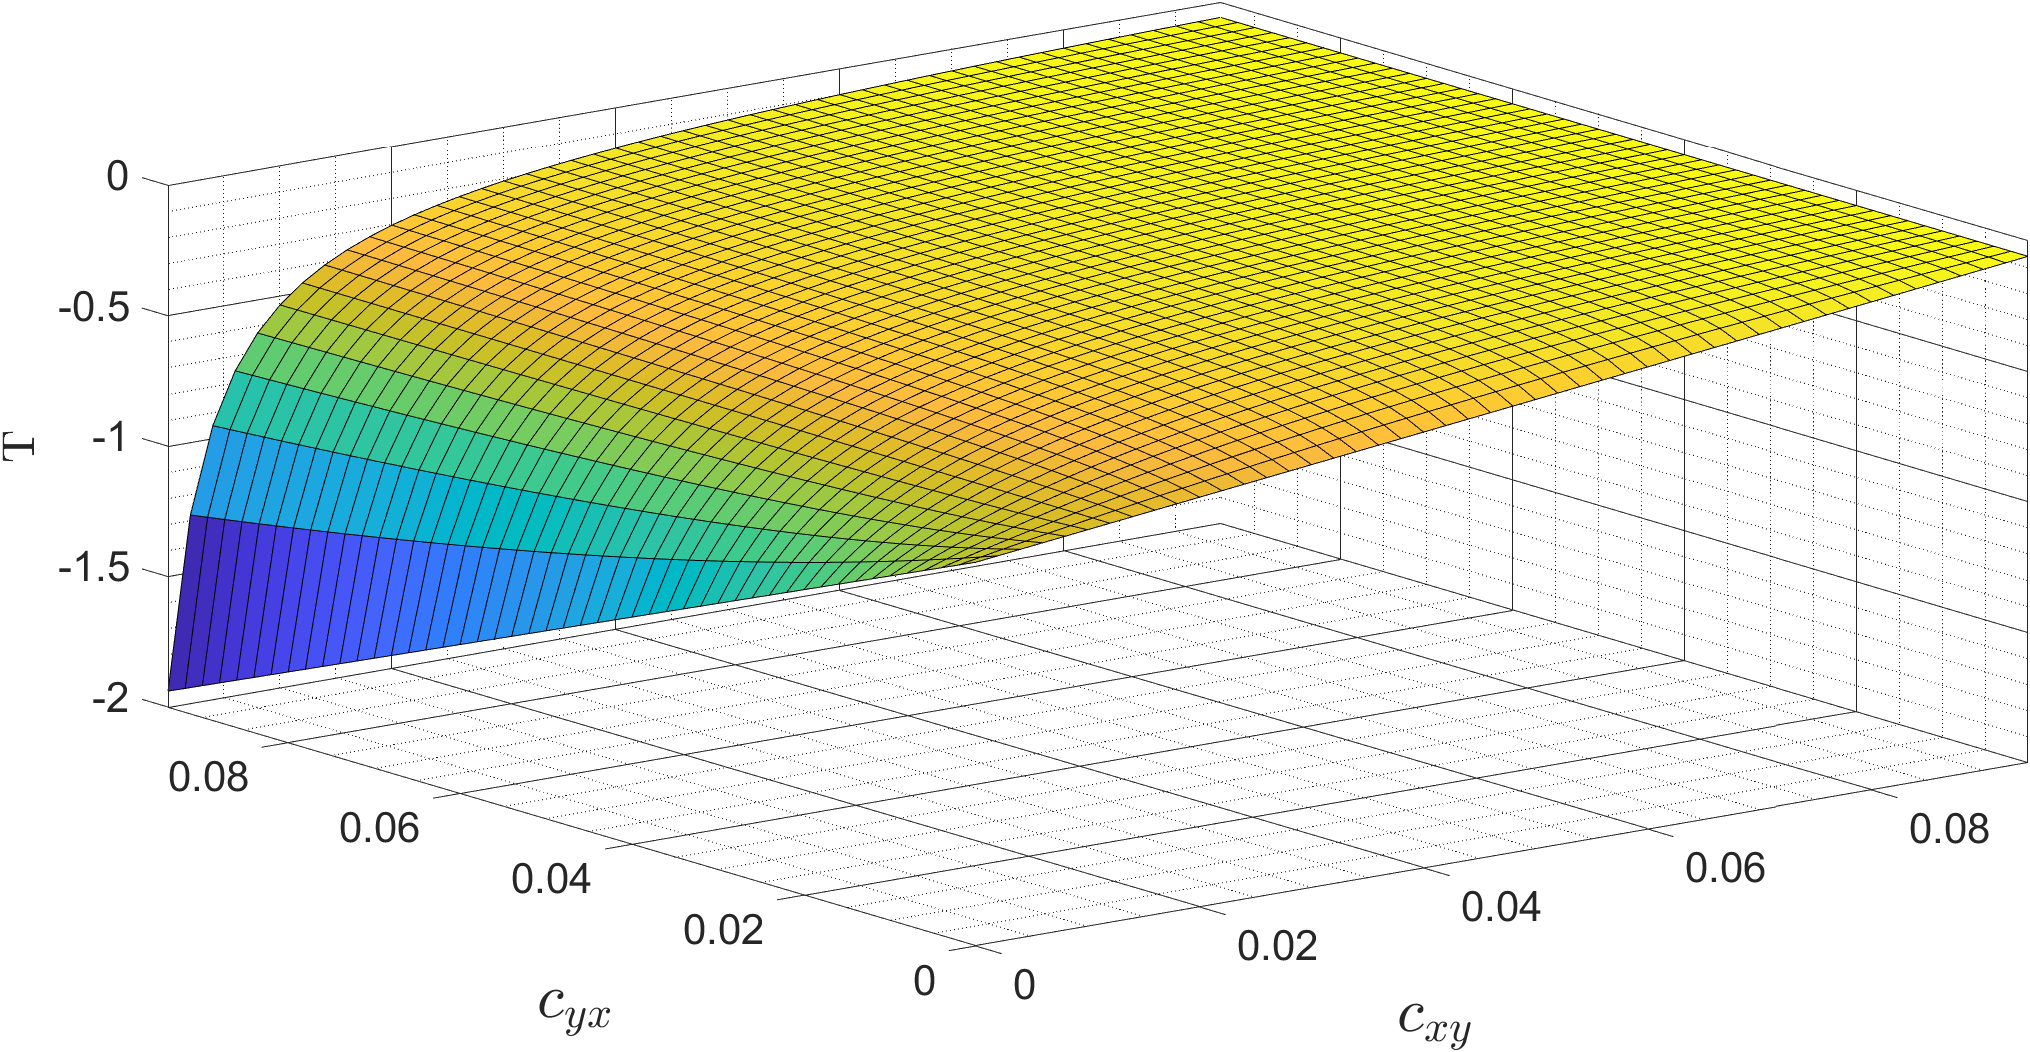
\includegraphics[width=14cm]{Pictures/Stability/Trace.png}
% \end{figure}
% \begin{figure}[H]
%     \centering
%     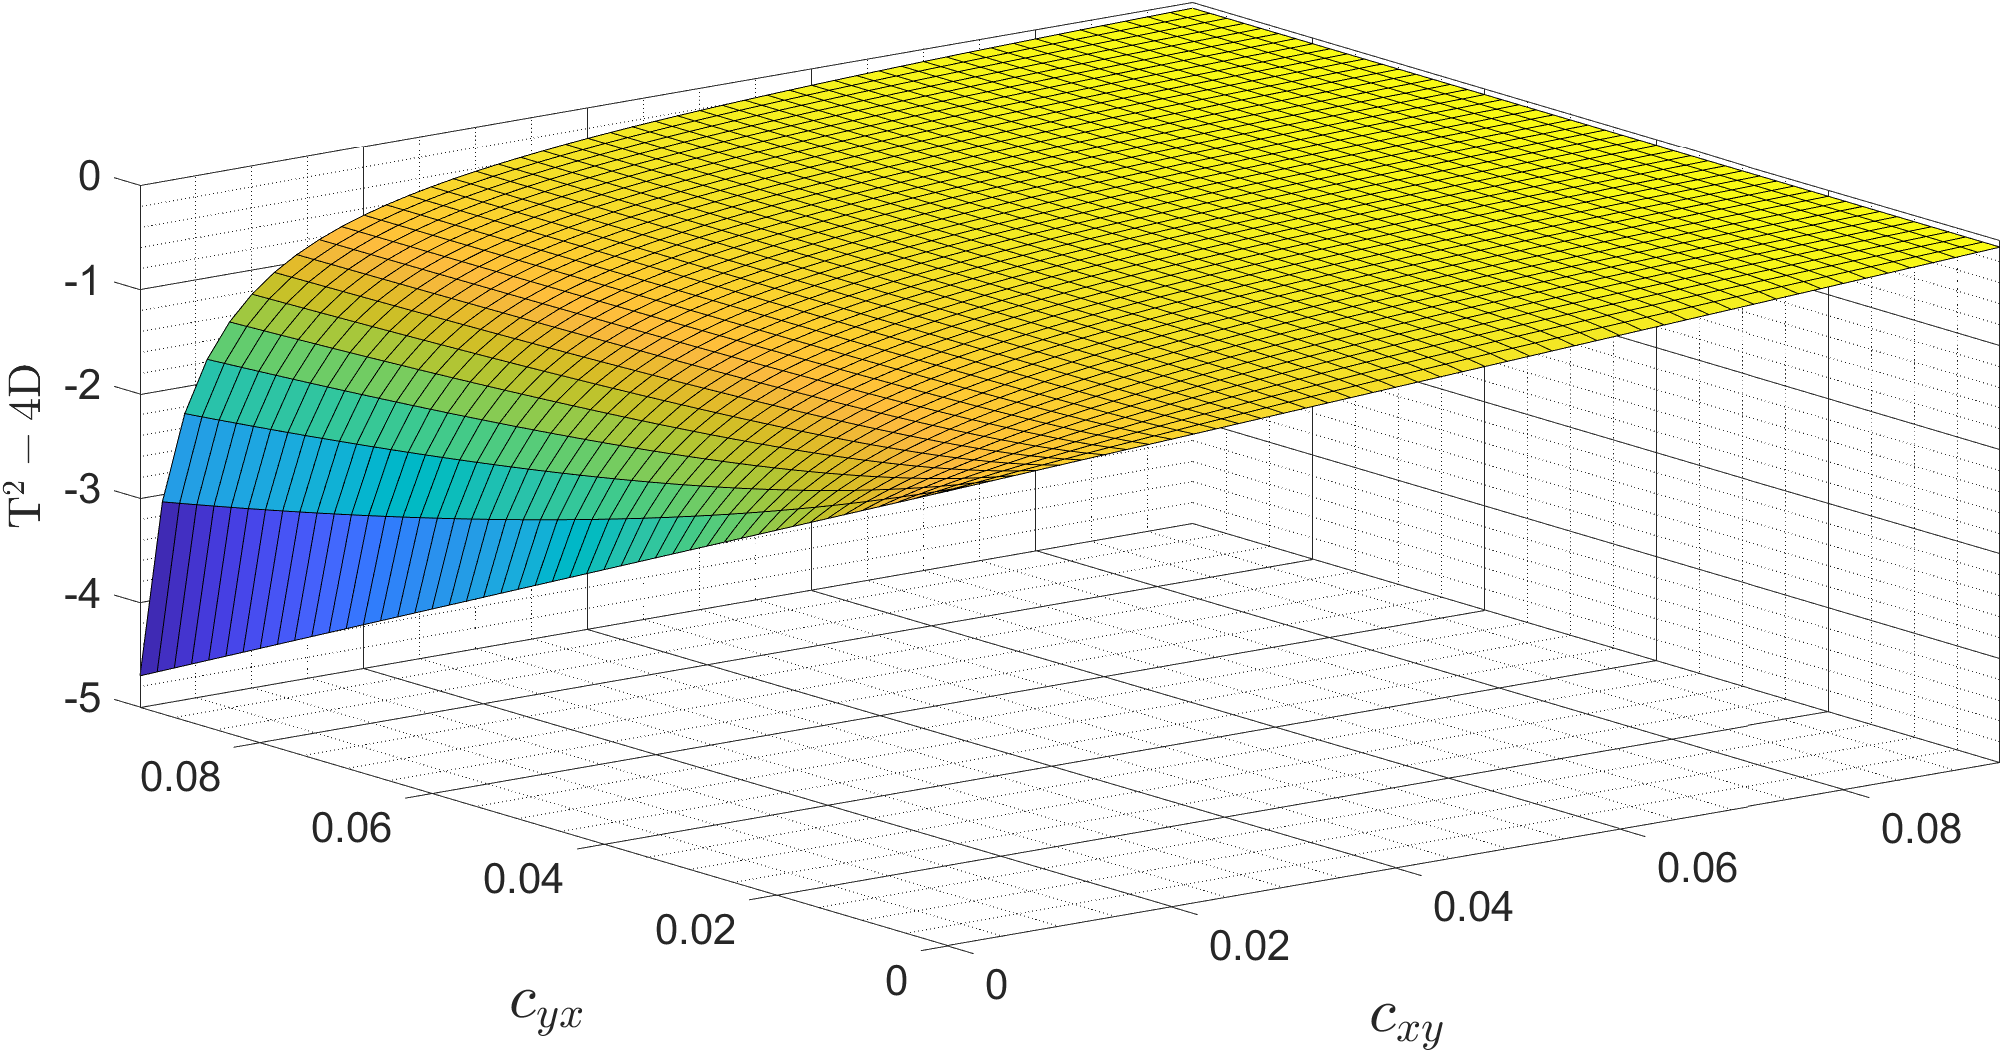
\includegraphics[width=14cm]{Pictures/Stability/Discriminant.png}
%     \caption{The graphs above are the trace and discriminant of $\displaystyle J_{(x^*_4,y^*_4)}$ for different values of the parameters $c_{yx}$ and $c_{xy}$.}
%     \label{fig:TraceDiscriminant}
% \end{figure}
% Notice that the values for the trace and discriminant are always negative for all $c_{yx}$ and $c_{xy}$ that belong in their constraints.
% Now, looking at these figure from a top-down view will provide a clear outline of which $c_{yx}$ and $c_{xy}$ values to test.
% \begin{figure}[H]
%     \centering
%     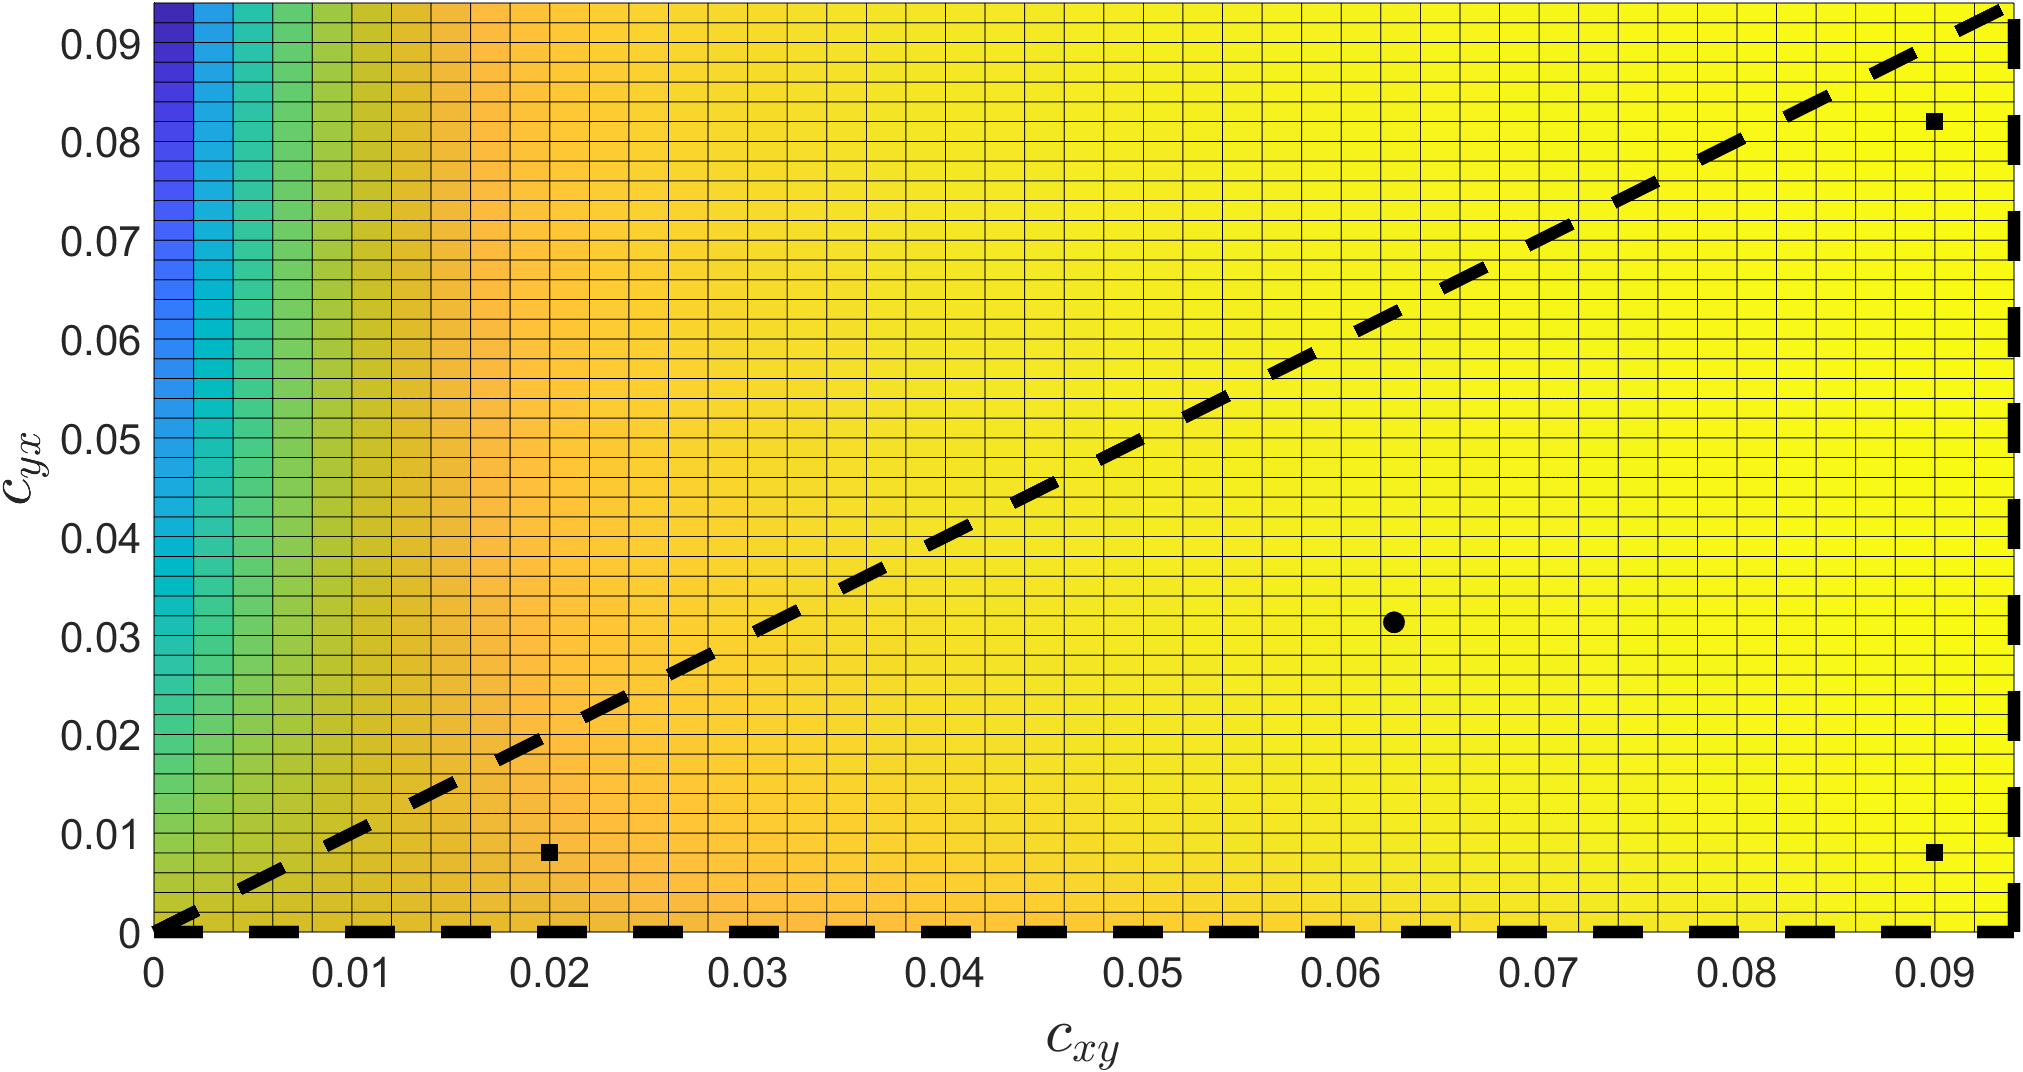
\includegraphics[width=14cm]{Pictures/Stability/TraceTopDown.png}
% \end{figure}
% \begin{figure}[H]
%     \centering
%     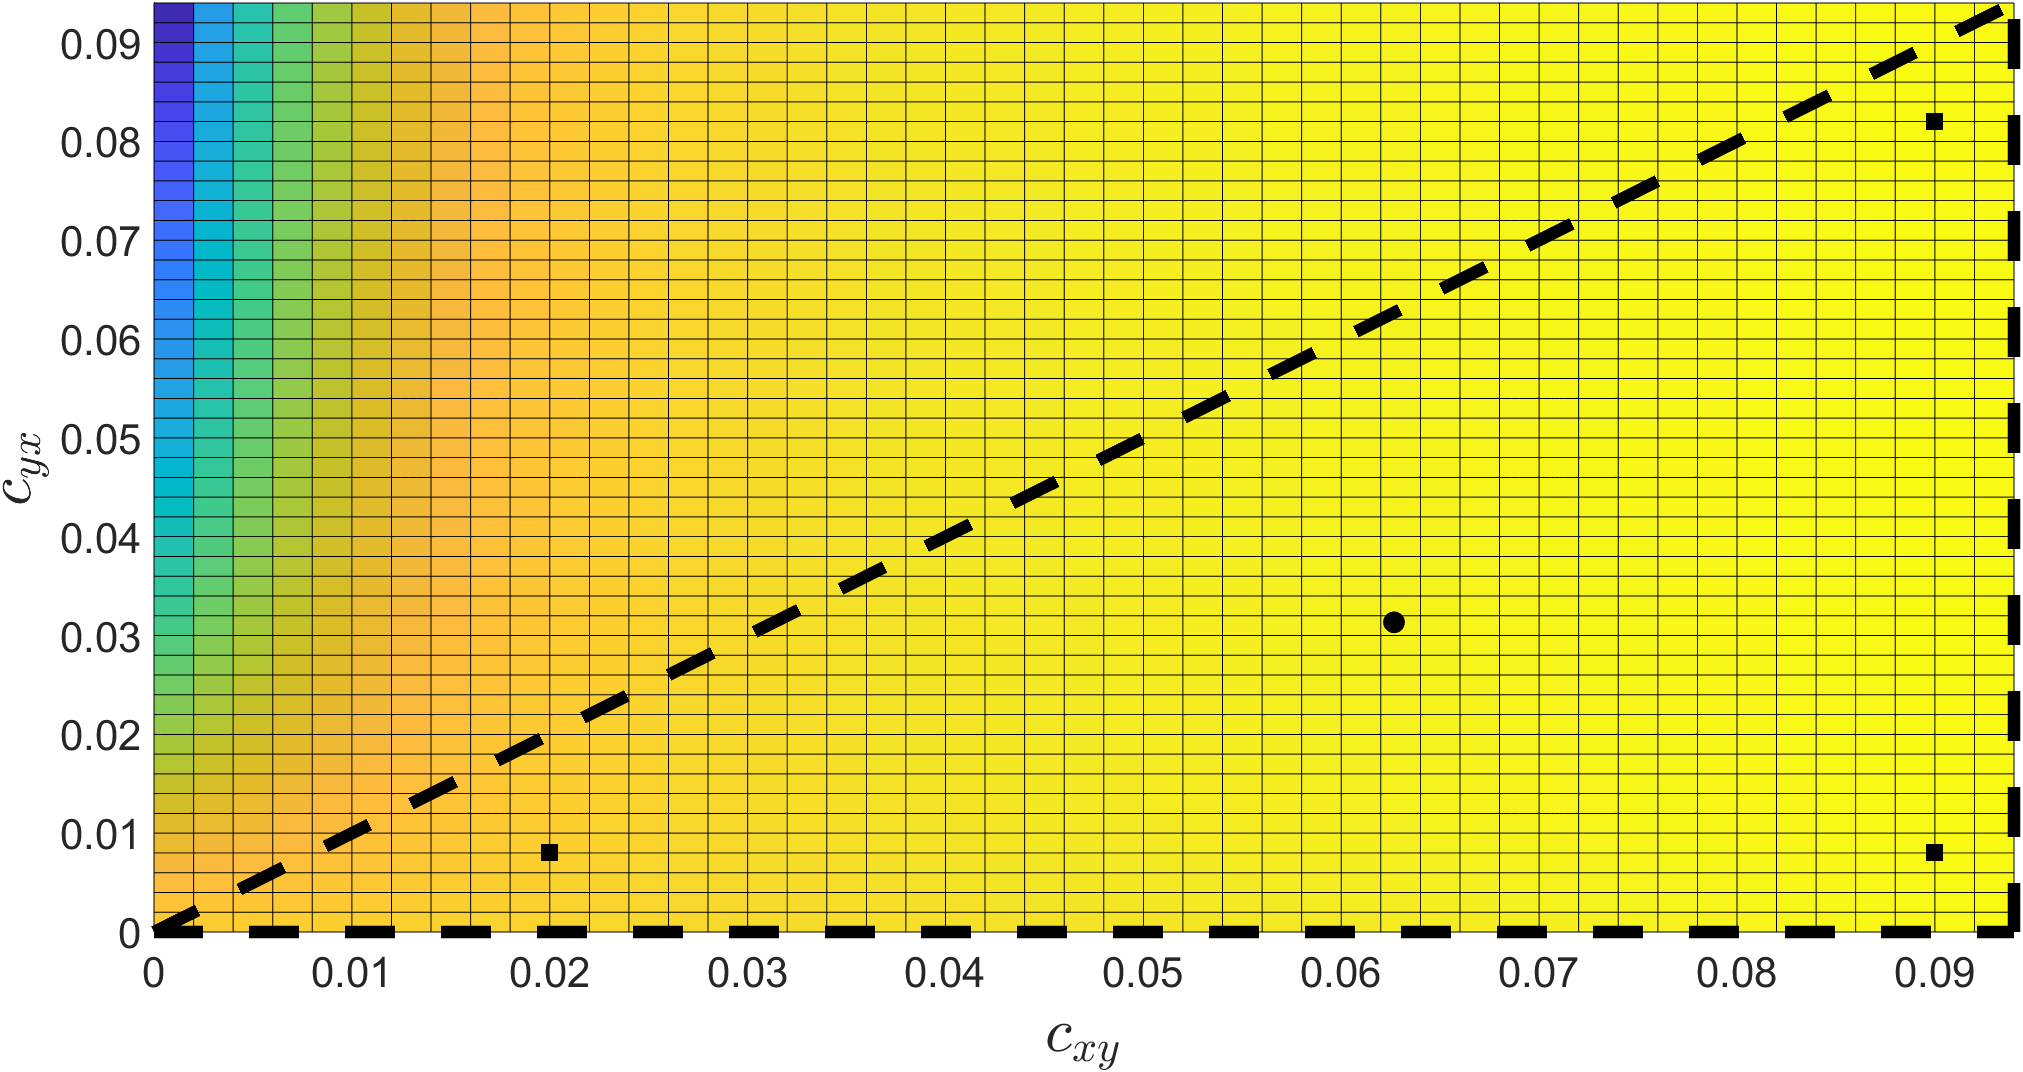
\includegraphics[width=14cm]{Pictures/Stability/DiscriminantTopDown.png}
%     \caption{Top-down view of \figureautorefname~\eqref{fig:TraceDiscriminant}. The points inside the right triangle are all values that satisfy the constraints of parameters $c_{yx}$ and $c_{xy}$. The right triangle's center of mass is marked with a black dot at the coordinate point $(0.0627,0.0313)$.}
%     \label{fig:TraceDiscriminantTopDown}
% \end{figure}
% In the figure above a region is drawn where all $c_{yx}$ and $c_{xy}$ satisfy their constraints.
% Now, testing different $c_{yx}$ and $c_{xy}$ values will illustrate how different interaction rates will effect the outcome of the each species' population.
% The values chosen for $(c_{xy},\;c_{yx})$ are $(0.02,\;0.008)$, $(0.09,\;0.008)$, $(0.09,\;0.082)$, and $(0.0627,\;0.0313)$. These pair of interaction parameters can be seen plotted on the figure above.
% To compare each of the parameters, we plot the solutions to \equationautorefname~\eqref{eq:AutonomousSystemODEs}, where the brown bear population is along the y-axis and the salmon population is along the x-axis as shown below for each pair of parameters.
% \begin{figure}[H]
%     \centering
%     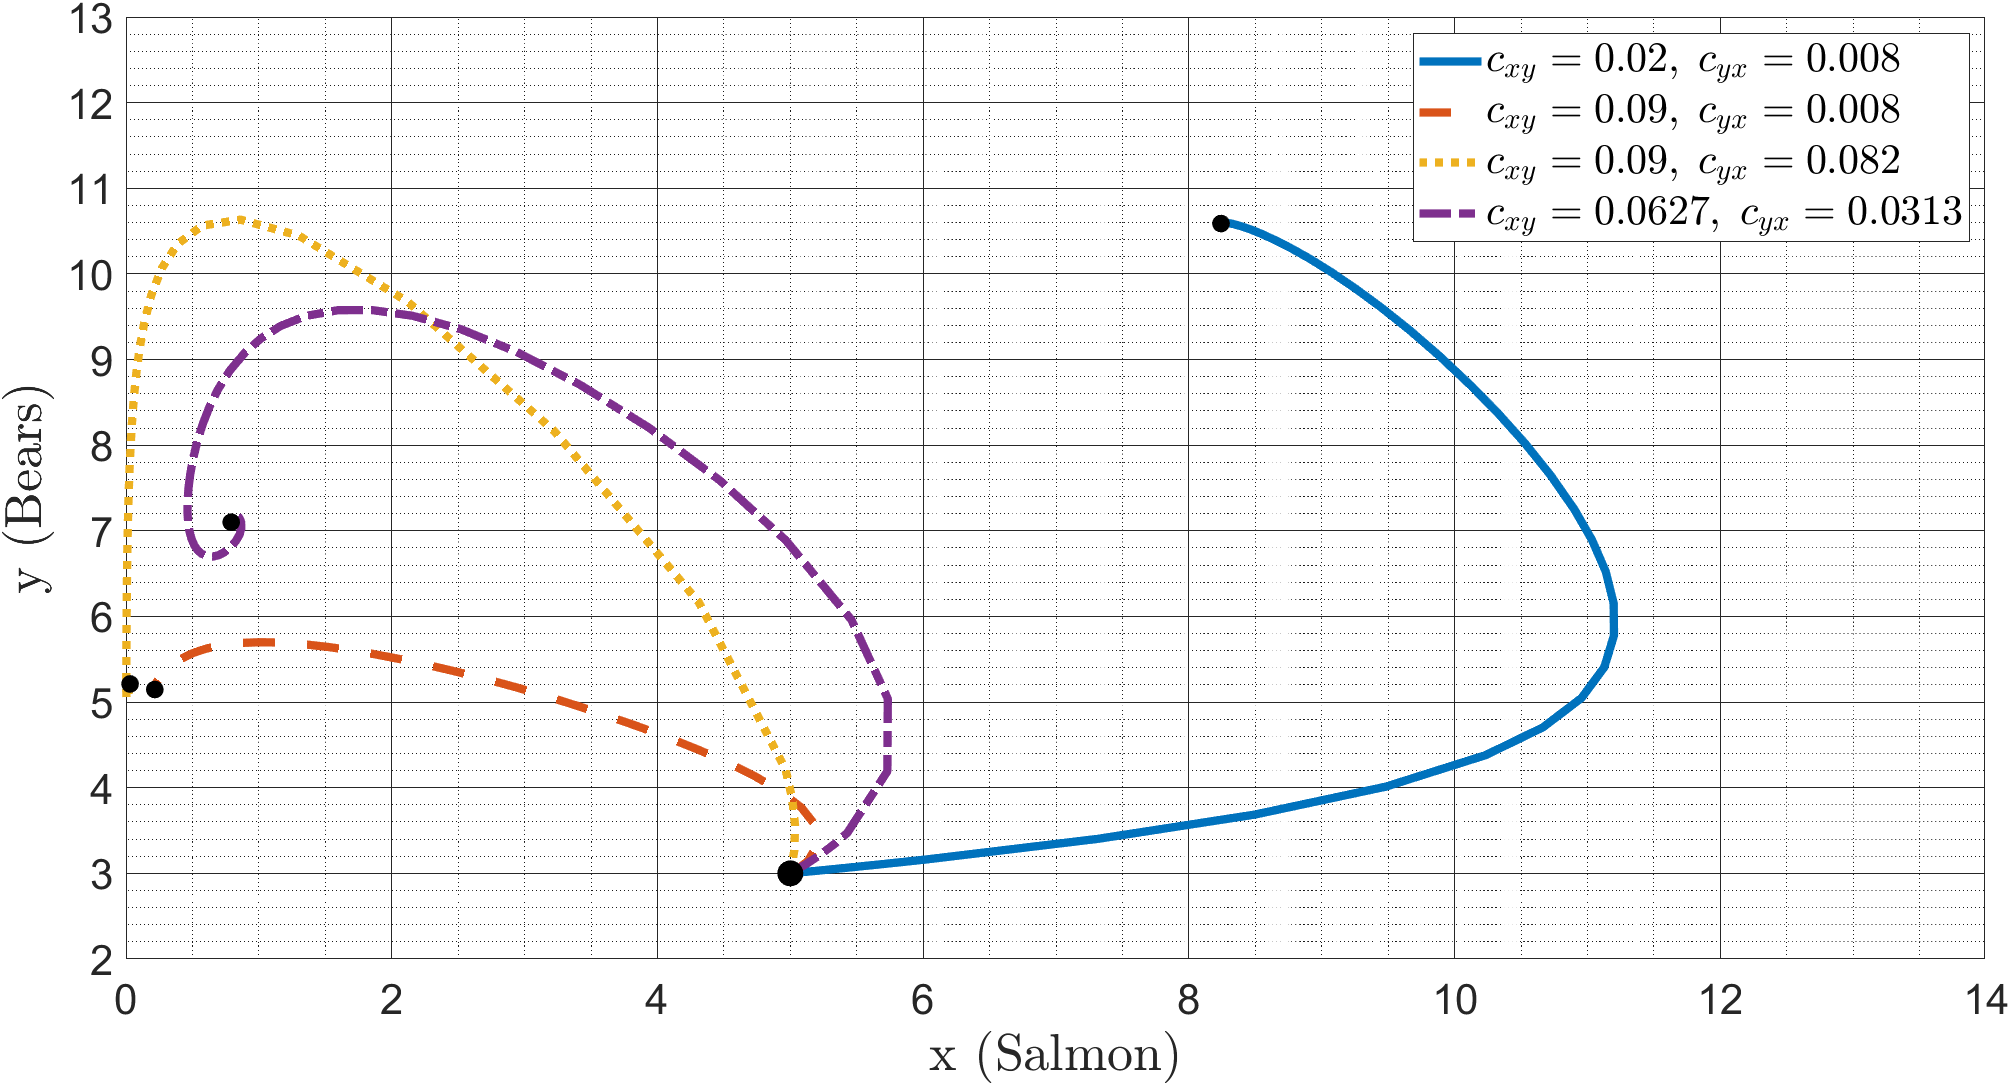
\includegraphics[width=14cm]{Pictures/Stability/SolutionsAutonomousModel.png}
%     \caption{Compares the effect of different interaction rates on the autonomous model, \equationautorefname~\eqref{eq:AutonomousSystemODEs}, where the initial conditions are $x_0 = 5$ and $y_0 = 3$.}
%     \label{fig:SolutionsAutonomous}
% \end{figure}
% The graph above shows that each of these parameters effects the location of the critical point, $(x^*_4,y^*_4)$ as well as the oscillations of the populations.
% We chose the initial conditions, $x_0 = 5$ and $y_0 = 3$, to illustrate the dramatic difference in interaction parameters.
% When $c_{xy}$ is large, the salmon population dies off, and when $c_{yx}$ is large, the brown bear population increases faster before converging near its carrying capacity.
% Lastly, when the pair of parameters is equal to the right triangle's center of mass in \figureautorefname~\ref{fig:TraceDiscriminantTopDown}, the population oscillates and converges to its critical point $(0.61,7.19)$.
% We will be using $c_{xy}=0.0627$ and $c_{yx}=0.0313$ to represent the interaction rates of the two species for \equationautorefname~\eqref{eq:AutonomousSystemODEs} because with these parameters the populations oscillate similar to what is expected in the real world.
% So, with all the parameters selected, the solutions to the autonomous model, \equationautorefname~\eqref{eq:AutonomousSystemODEs}, with respect time is shown below.
% \begin{figure}[H]
%     \centering
%     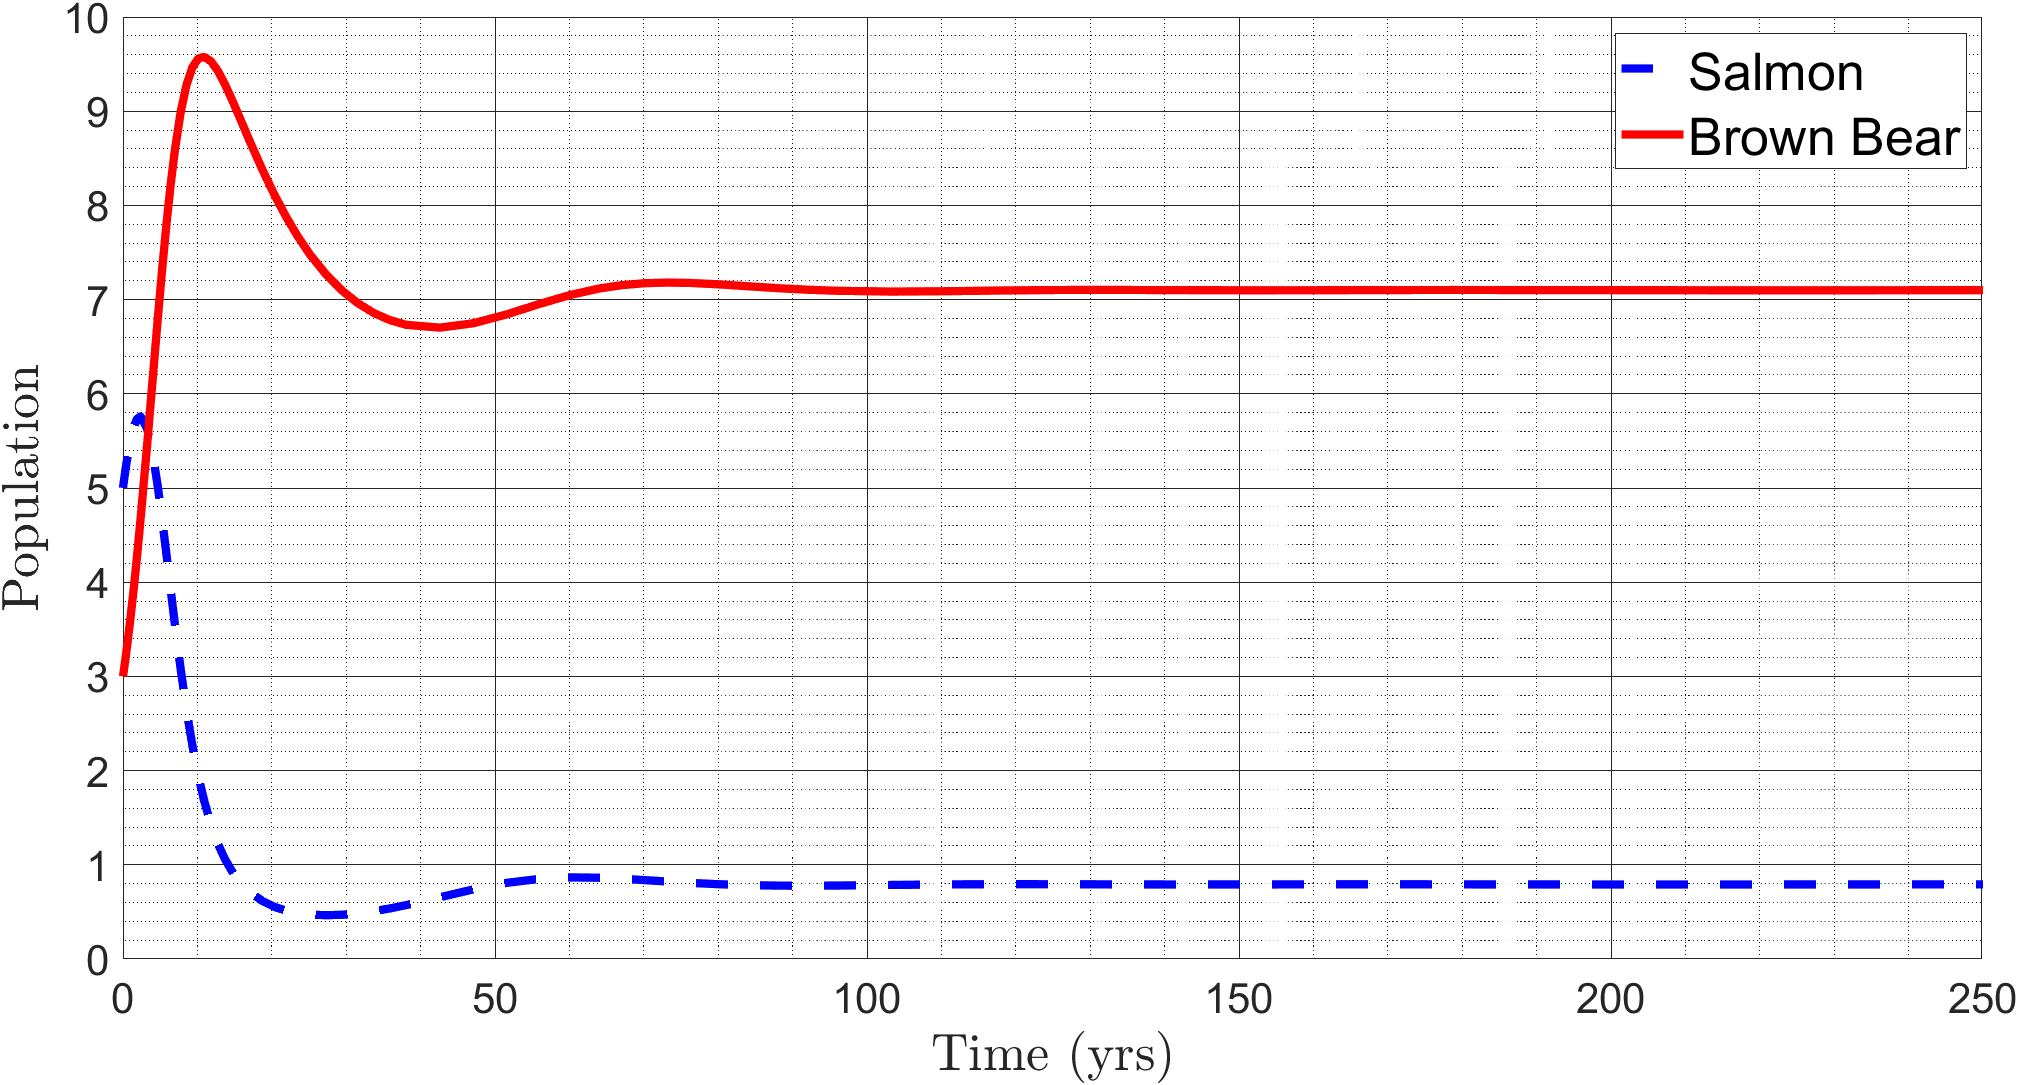
\includegraphics[width=14cm]{Pictures/System ODEs/AutonomousModelRespectTime.png}
%     \caption{Plot of  the solutions to the autonomous model, \equationautorefname~\eqref{eq:AutonomousSystemODEs}, with respect to time.}
%     \label{fig:SolutionsNonAutonomous}
% \end{figure}
% In the figure above, both populations briefly increase before changing directions and oscillating toward their equilibrium points.
% Based on this figure, the brown bear population will quickly overtake the salmon population, forcing the salmon near regional extinction.



% Now, we can compare these results to the system of ODEs, with the proposed growth rate, $G(t)$, shown below.
% \begin{equation}\label{eq:Non-AutonomousSystemODEs}
%     \begin{aligned}
%     \frac{dx}{dt} &=G(t)x\left(1-\frac{x}{K_x}\right) - c_{xy}xy,\\[.4cm]
%     \frac{dy}{dt} &=r_yy\left(1-\frac{y}{K_y}\right) + c_{yx}xy.
%     \end{aligned}
% \end{equation}
% Now, using the same parameters for the autonomous model, \equationautorefname~\eqref{eq:AutonomousSystemODEs}, we compare different initial conditions to analyze the stability of the model.
% \begin{figure}[H]
%     \centering
%     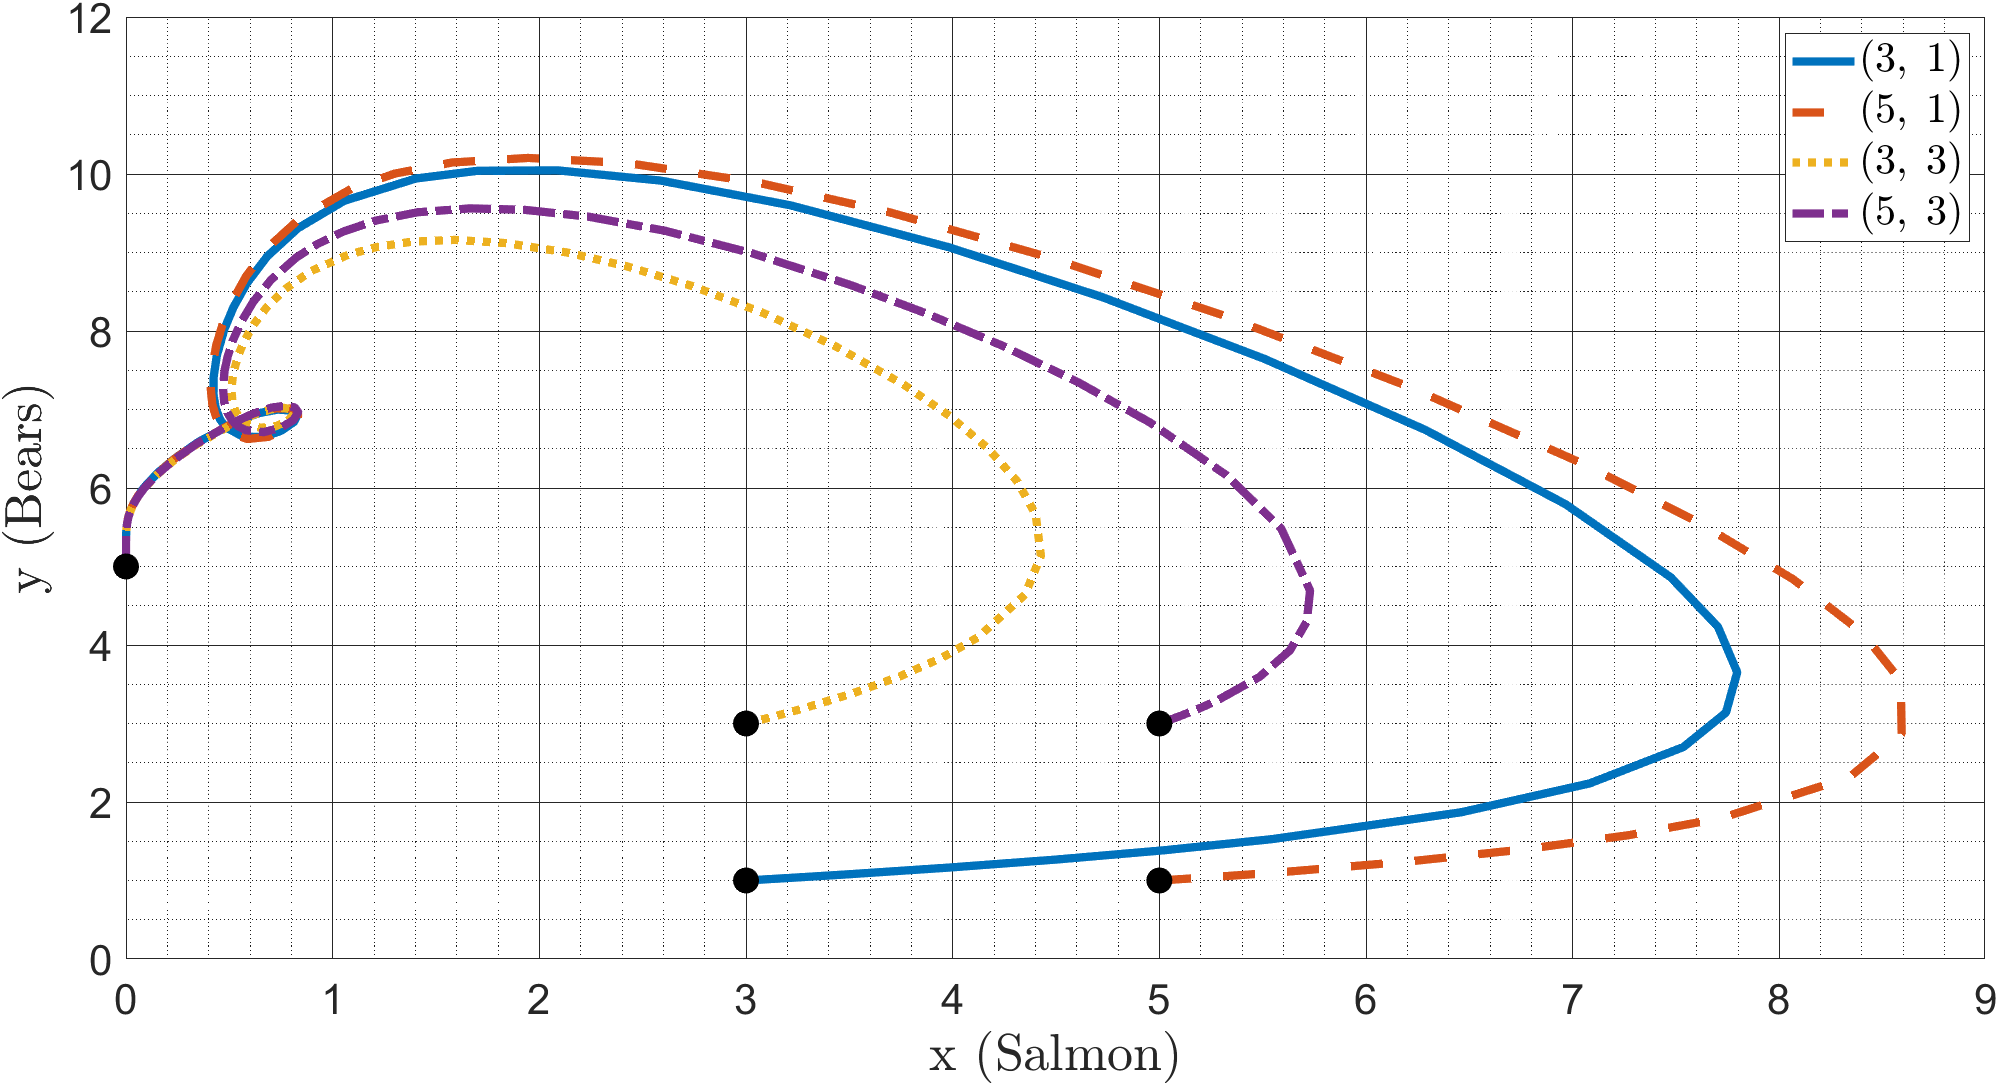
\includegraphics[width=14cm]{Pictures/Stability/SolutionsNonAutonomousModel.png}
%     \caption{Compares the solutions to the non-autonomous model, \equationautorefname~\eqref{eq:Non-AutonomousSystemODEs}, with different initial conditions.}
%     \label{fig:Non-AutonomousSystemODEs}
% \end{figure}
% As expected the salmon population converges to zero as seen in \figureautorefname~\eqref{fig:SalmonWithRepoFun}, resulting in the brown bear population converging to their carry capacity.
% When the salmon population dies off, the interaction terms in the model will approach zero and eventually the behavior of the brown bear species will be represented by its logistic equation, \equationautorefname~\eqref{eq:LogBear}.
% Lastly, in the graph below, we compare the results to the autonomous and non-autonomous model.
% \begin{figure}[H]
%     \centering
%     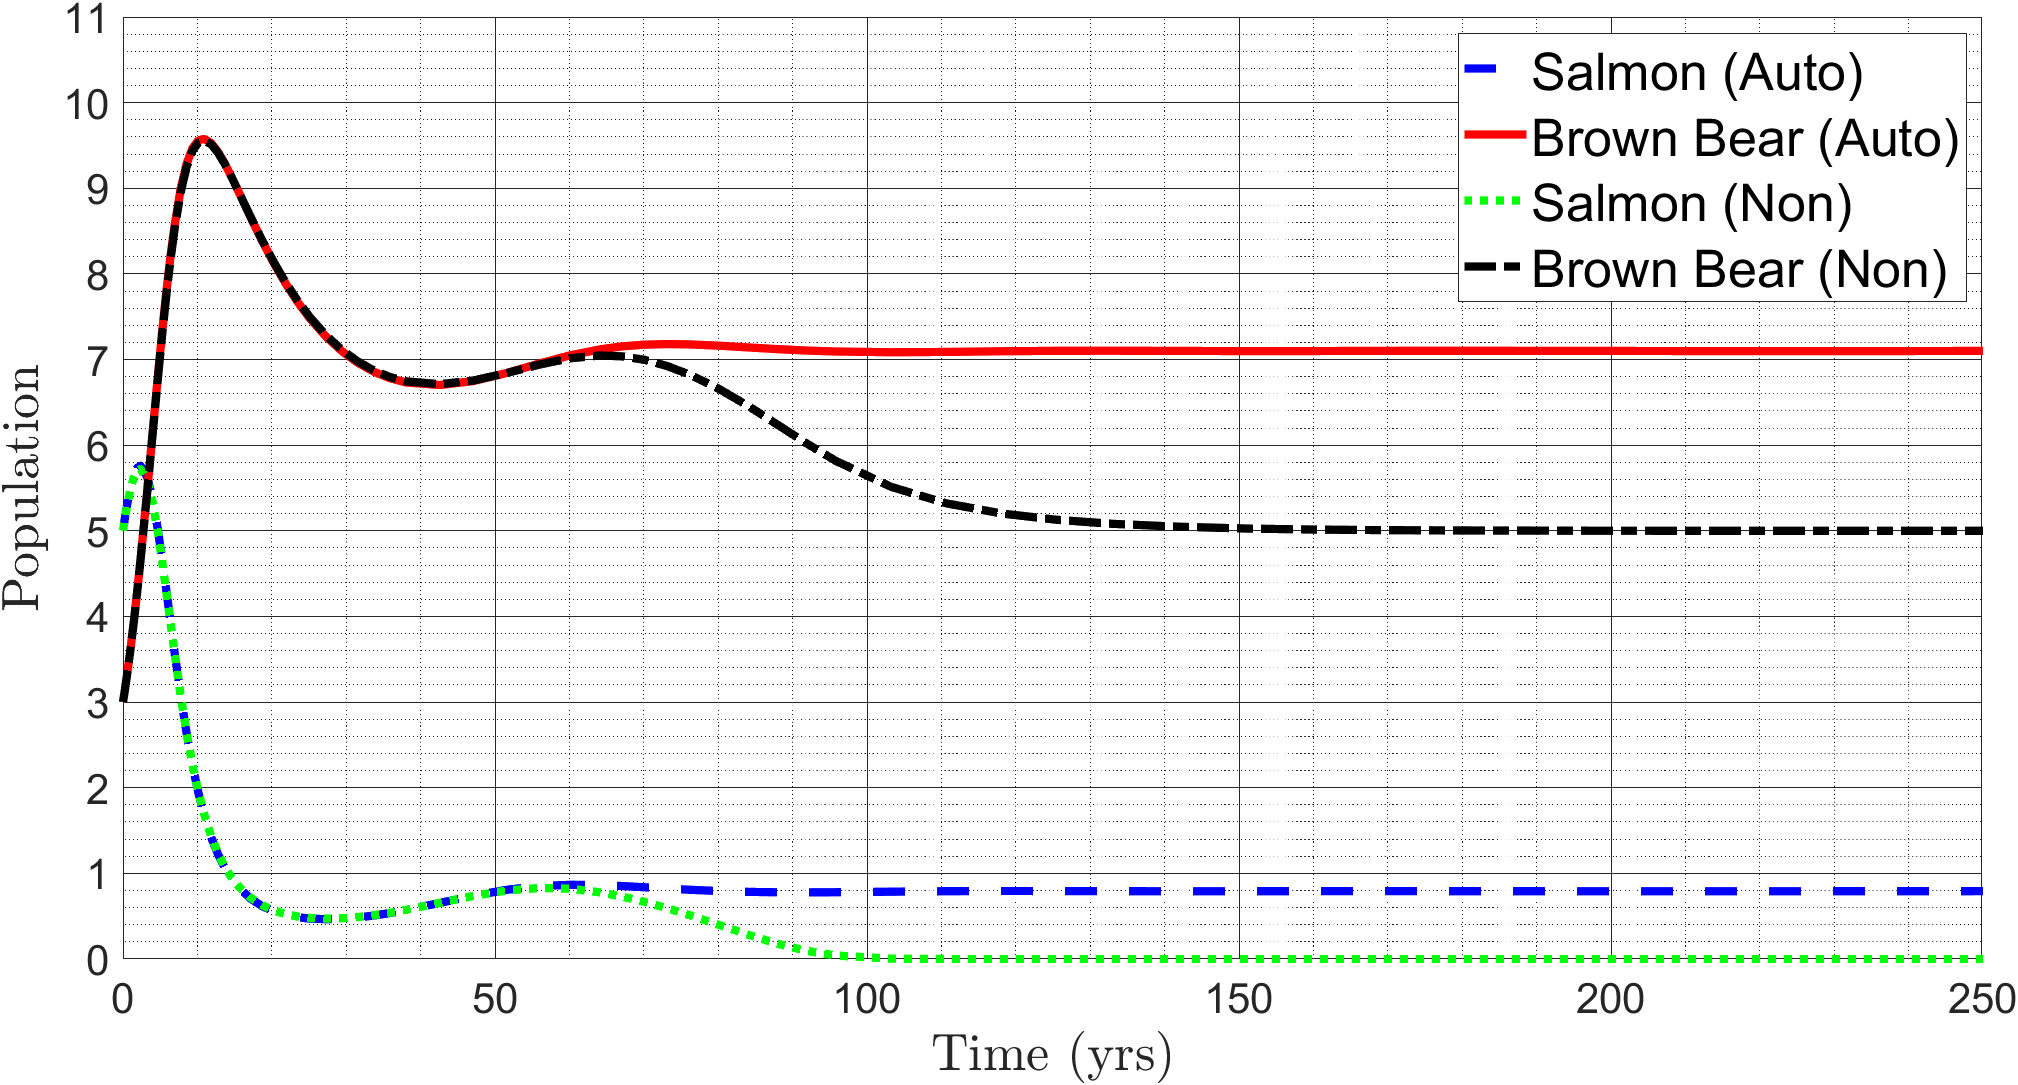
\includegraphics[width=14cm]{Pictures/System ODEs/AutonomousVsNonautonomous.png}
%     \caption{Plot of the solutions to the autonomous and non-autonomous model with respect to time.}
%     \label{fig:AutonomousVsNon-Autonomous}
% \end{figure}
% Initially, the two models follow the same path, but after approximately 65 years, the curves begin to deviate.
% According to our temperature function, \equationautorefname~\eqref{eq:sstmodel}, the projected Alaskan river temperature in 65 years is $T(65)\approx14.7^{\circ}$C.
% Therefore, the graph illustrates that soon after the river temperature leaves the optimal range, the difference in the outcomes of the species' populations becomes prominent.
% The non-autonomous model shows similar trends to the autonomous model, but ultimately resulting in the salmon population dying off and the Alaskan brown bear population converging to its carrying capacity.










% \begin{equation*}\scalebox{1.4}{$
%     \begin{array}{cc}
%          x^*_4 = \frac{\ln(R(T))*\frac{r_y}{K_y} - c_{xy}*r_y}{c_{xy}*c_{yx}+\frac{\ln{(R(T))}*r_y}{K_x*K_y}} & y^*_4 = \frac{\ln(R(T))*c_{yx}+\frac{\ln(R(T))}{K_x}*r_y}{c_{xy}*c_{yx}+\frac{\ln{(R(T))}*r_y}{K_x*K_y}} 
%     \end{array}$}
% \end{equation*}